\chapter{Monte Carlo Generators}
\label{cap3}


\textit{As we have seen in the collisions between high energy protons hundreds of particles are generally present in the final state.
Given the complexity of the events it is necessary to use Monte Carlo generators, i.e. programs that allow to simulate the realistic result of the collisions assuming a certain model for the processes involved. In this chapter are described the various stages beyond the Monte Carlo events simulation. In particular I have participated personally to the Monte Carlo production and validation for the CMS collaboration.  }

\section{General Overview}
The use of Monte Carlo generators is necessary because it is impossible to predict what happens event-by-event: in fact,  in quantum mechanics we can only calculate the probability of having a certain result.
The simulation of an event is carried out in successive steps \cite{Sjostrand:2006su, Buckley:2011ms}, as schematized in Fig.~\ref{qqqq}, thus subdividing the problem into several parts of lower complexity.


\begin{figure}
\centering
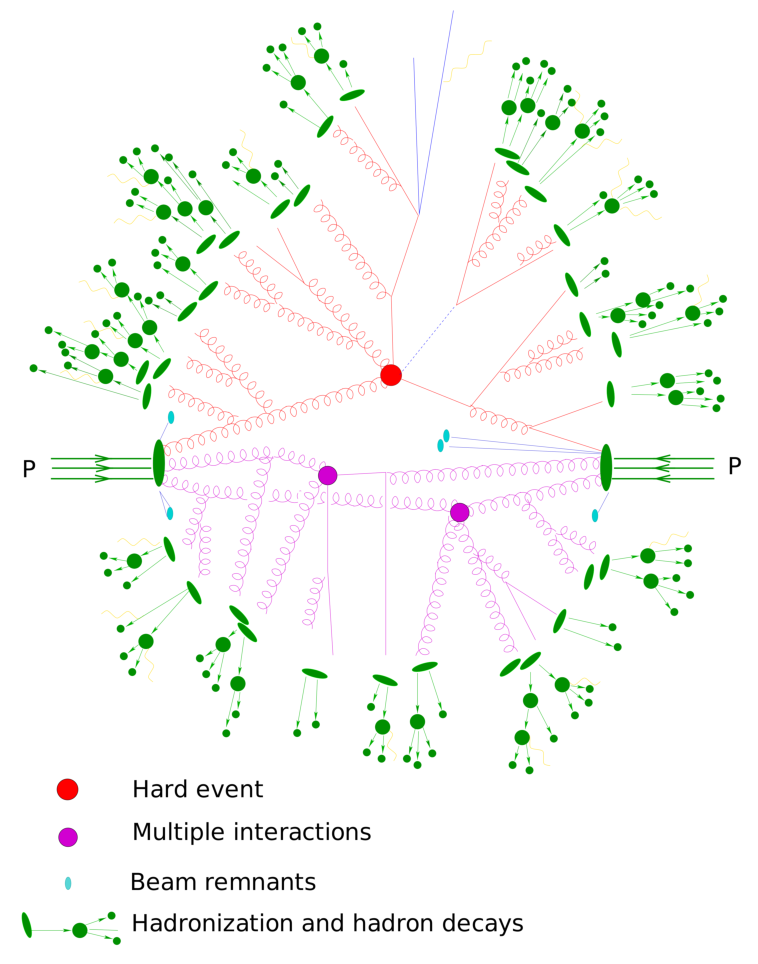
\includegraphics[scale= 1]{../Cap3/Fig_MC/generalMC}
\caption{Schematic representation of an event generated within an event generator. The partons coming from the protons indicative participate in both the hard process and multiple interactions. Subsequently there is the hadronization.}
\label{qqqq}
\end{figure}
The various steps are summarized here:
\begin{itemize}

\item Hard process: the incident protons are composed by  partons (quarks and gluons) and the hard process consists in a collision between two partons, coming from different hadrons. The  matrix element of the process is evaluated perturbatively and often only the lowest perturbative order, called leading order (LO), is calculated.
\item Parton shower: the incoming or outgoing partons participating in the hard process can emit gluons. In fact, in analogy with the electromagnetic interaction, a particle with an accelerated color charge can radiate for the bremsstrahlung.
The gluons in turn, can produce quark-antiquark pairs thus generating the parton showers.
The emission of additional partons takes place mainly in the collinear space respect to the initial parton and  progressively with less energies.
In the final state there will be a set of partons, called jet, located in the collinear with respect to the initial parton.
This probabilistic process can be simulated as a Markov process and is implemented in the parton shower algorithms we will discuss later.

\item Multiple interactions: in a single collision, it may happen to have more pairs of partons interacting. In this case it is said that there are multiple interactions in addition to the hard process.

\item Hadronization: in the evolution of the event the partons are generated with gradually lower relative momenta. 
For momentum values of 1 about GeV the confinement forces prevail. At these energy scales, the perturbation theory fails in the description, so we resort to non perturbative models which describe the formation of real hadrons. This hadronization process  preserves the jet structure which can therefore be observed experimentally.

\item Decaying of unstable particles: many of the particles produced in the primary process are unstable and they  decay unless they interact before with the detector.

\end{itemize}

In the  Monte Carlo simulation  all these steps are considered sequentially: the result of each step is the starting point of the next.
At the end, in a single event, there are hundreds of particles each of which has a dozen degrees of freedom (mass, flavor, impulse, average life, spin, vertex production, etc.), so there is a  high number of parameters that came into play and must be simulated for each event.
The final aim is to provide a realistic description of what happens in high-energy collisions, in order to compare the Monte Carlo model with the experimental data.
Schematically, the cross section of the final state is given by,
\begin{equation}
 \sigma_{final \: state}=\sigma_{hard \: process} \cdot \: \mathcal{P}_{tot, \:hard \: process \rightarrow final \:state} \: \mbox{,}\end{equation}
integrated over the total phase space and summed over all possible final states (e.g. the production of two or more jets). This is the measurable quantity associated with the hard process. \\




\section{Hard process}

In many processes of interest to LHC, high momenta come into play, to produce high mass particles or  energetic jet. The simulation of these events is the main goals of the Monte Carlo generators.
The cross section for a scattering $ ab \rightarrow n $ process is given \cite{Buckley:2011ms} by,
\begin{eqnarray}
 \sigma & = & \sum_{a,b}  \int_{0}^{1} \, dx_{a} dx_b \int f_{a}^{h_1} (x_a , \mu_F) f_{b}^{h_2} (x_b , \mu_F) \: d \hat{\sigma}_{ab \rightarrow n}(\mu_F , \mu_R)  \nonumber \\
& = & \sum_{a,b}  \int_{0}^{1} \, dx_{a} dx_b \int d \Phi_n  f_{a}^{h_1} (x_a , \mu_F) f_{b}^{h_2} (x_b , \mu_F) \nonumber \\
 & \times& \frac{1}{2\hat{s}} 
 | \mathcal{M}_{ab \rightarrow n} 
(\Phi_n , \mu_F , \mu_R)|^2  \: \mbox{,} \end{eqnarray}
where
\begin{itemize}
\item $f_{a}^{h} (x , \mu)$ are the parton density functions (PDF) that depend on the $x$ fraction of the parton $a$'s energy (Bjorken variable) respect to the 
hadron $h_i$ ($i=1,2$), and on the $\mu_F $ factorization scale, App~\ref{pdfa}.
\item $\hat {\sigma}_ {ab\rightarrow n} $ is the partonic cross section of the process $ ab \rightarrow n $.
The total differential cross section is given by the product of the corresponding square matrix element, $ | \mathcal {M}_{ab \rightarrow n} |^2 $, 
with  the incident particle flow $ 1 / (2 \hat{s}) = 1 / (2 x_a x_b s) $, where $ \sqrt{s} $ is the energy of the system's center of mass.
\item The matrix element $| \mathcal{M}_{ab \rightarrow n}  (\Phi_n , \mu_F , \mu_R) |^2 $  can be written as the sum on all Feynman diagrams,
\begin{equation}
\mathcal{M}_{ab \rightarrow n}= \sum_{i} \mathcal{F}_{ab \rightarrow n}^{(i)} \: \mbox{.} \end{equation}
\item $d\Phi_n$ it is the phase space differential for $ n $ particles in the final state.
\end{itemize}
The phase space will not be all physical space  but will contain cuts for two reasons: the first is that  the cuts will reflect the geometry and acceptance of the detector; the second because it is necessary put a cut on the transverse impulse of the particles produced in the process to avoid divergences in the calculation of the cross section \footnote {You can imagine having a singularity similar to that  in classical Coulomb scattering.}.
In general, the calculation of the matrix element would require the calculation of all the Feynamn diagrams which  grow in a factorial way (Fig.~\ref{fatt}) with the number of particles in the final state.
\begin{figure}[h]
\centering
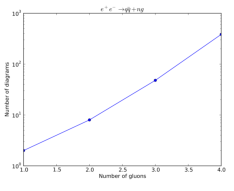
\includegraphics[scale= 2.5]{../Cap3/Fig_MC/fattoriale}
\caption{ Trends in the number of Feynman diagrams as the number $ n $ of gluons increases in the process $e^+ e^- \rightarrow q \bar{q} + ng$.}
\label{fatt}
\end{figure}
Usually the  Monte Carlo events generators can compute the matrix element at the leading order for the Standard Model $2 \rightarrow 1$,  $2 \rightarrow 2$  
and  $2 \rightarrow 3$ \cite{bib:madgraph} processes.  \\
However, if we stop at the first perturbative order, we would have only a rough description of the process: in fact, subsequent orders involve important corrections both to the shape of the distributions and to the total cross section. LO is useful for a first study but  it is important to evaluate next-to-leading-order (NLO) \footnote{For some particularly important processes, for example $ gg \rightarrow H $, the next-next-to-leading-order (NNLO) calculations are even available.}. \\
The cross section calculated at the NLO is composed of three parts: the LO part or Born, by the real and by the virtual part of the emission corrections (Fig. \ref{nlofig}),
\begin{equation}
 \label{xsecNLO}
 d\sigma^{NLO} =  d \tilde{\Phi}_n [\mathcal{B} (  \tilde{\Phi}_n  ) + \alpha_s \mathcal{V}(  \tilde{\Phi}_n  ) ] +  d \tilde{\Phi}_{n+1} \alpha_s \mathcal{R}(\tilde{\Phi}_{n+1}  ) \: \mbox{,}   \end{equation}
 where $\mathcal{B}$, $\mathcal{R}$ and $\mathcal{V}$  denote the Born, the real  and the virtual part respectively. The integral must be made on the $ n $ or $ n + 1 $ final state particles and on the Bjorken variables related to the incident partons.
Consider, in the Born approximation, the process  $ 2 \rightarrow 2 $. If you want to go to the next order, NLO, you have to keep the element with an additional parton in the final state, the $ 2 \rightarrow 3 $ process, and virtual correction with a loop in the $ 2 \rightarrow 2 $ process.
It should be noted that the cross-section for processes of the type $ 2 \rightarrow 3 $ is divergent when the energy of one of the partons tends to zero (soft divergence) or when two partons are collinear (collinear divergence).
\begin{figure}
\centering
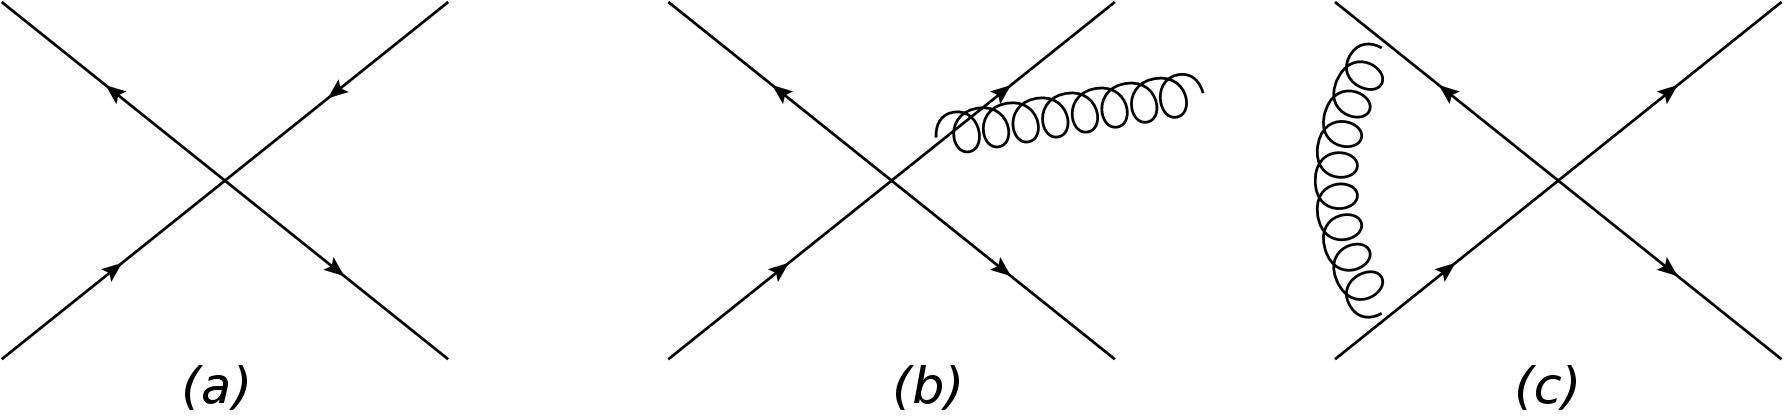
\includegraphics[scale=0.22]{../Cap3/Fig_MC/nlo2}
\caption{ Examples of Feynman diagrams (a)  Born, (b) real, (c) virtual. }
\label{nlofig}
\end{figure}
\section{Parton shower}
\label{ps}
In a collision between partons a charge of color is accelerated, so there will be bremsstrahlung emission. When studying a process of the type $ 2 \rightarrow n $, where $ n $ represents the number of partons in the final state, the LO matrix elements (called tree-level) will have divergences in the collinear  and 
soft case. In particular, the processes that suffer from this type of divergence are $ q \rightarrow qg $, $ \bar{q} \rightarrow \ bar{q} g $, $ g \rightarrow gg $: the first are similar processes to $ e \rightarrow e \gamma $ in QED, while the third is due to the fact that QCD is not an Abelian theory. The process $ g \rightarrow q \bar {q} $ does not have this type of divergence.
The divergences of the tree-level matrix element can be removed by introducing the virtual corrections into the calculation, but they will be in the next order; these calculations are therefore particularly complex and they are only possible for a limited number of processes. The parton shower \cite{Sjostrand: 2006su} algorithms offer an alternative and simple way to eliminate the collinear and soft divergences through:
\begin{itemize}
\item an iterative structure that combines the three states suffering from divergences in a single multi-partonic state,
\item the introduction of the form factor of Sudakov.
\end{itemize}
The incoming or outgoing partons, which are far (temporally) from hard process, are called on-shell. Indeed the module of their four-momenta   is equal to the mass at rest.
However, the closer one gets to the interaction,  the more  partons can be off-shell, i.e. the module of the their four-momenta does not correspond to the mass at rest due to the uncertainty principle ($ \Delta E \Delta t \sim \hbar $),. 
For this reason they are able to emit other partons and  the energy of emitted partons is higher if they are closer to the scattering.
If the emission occurs before the scattering, it is called initial state radiation (ISR), while after the interaction it is called final state radiation (FSR). \\
Each parton  is characterized by a  ``virtuality scale'' $Q^2$ that corresponds roughly to a shower temporal scale.
It is important to stress that different definitions are available for $Q^2$; however regardless of the chosen convention, the $ Q^2 $ scale increases as it approaches the hard process,  in the ISR, and decreases away, in the FSR. If we take the FSR,  the evolution starts at a $ Q^2_ {max} $ scale that is related to the hard process and it ends when a limit scale is reached, $ Q_0 $, which will be on the order of 1 GeV .\\
The most common choice used is to set  $Q^2=p^2=E^2- |\vec{p}\,|^2$. With this convention in a process of type  $a \rightarrow bc$, in FSR case, $Q^2 >0$, 
$Q$ is time-like, decreases until the limit scale $ Q_0 $ is reached.
The ISR case is complicated. In this case, if $c$ is an emitted parton that will not participated in the hard interaction, $a$ and $b$ are off-shell. The are space-like and in order to guaranteed the increase order of $Q^2$,  i.e. $ Q_b^2> Q_a^2 $, it is better to define  $ Q_i^2 = -m_i^2 $. In contrast $c$ is time-like 
Therefore its shower will evolve like that of the FSR.

\subsection*{Final State Radiation}
In the parton shower approach, the final state radiation  is modeled through a series of divisional processes of the type $ a \rightarrow bc $.   
This is evident from the process $q \bar{q}g$, Fig. \ref{nlofig} (b), where the first order matrix element  corrections  correspond to the emission of a gluon. 
The evolution of the shower is described by two parameters: the fraction of energy carried by one of the two outgoing partons, $ z = E_b / E_a $, and the order variable $ t $. As we said, a possible choice for $ t $ is the  virtuality $ Q_a^2 $ of the incoming parton.
In the  collinear limit the probability of division $d \mathcal{P}_{a \rightarrow bc}$, in  $z$ and $t=\ln(Q^2/\Lambda^2)$ is:
\begin{equation}
 d \mathcal{P}_{a \rightarrow bc}=  \frac{\alpha_{abc}}{2 \pi}\: {P}_{a \rightarrow bc} \:dt dz  \: \mbox{,} \label{prob}  \end{equation}
where $dt=\frac{d Q^2}{Q^2}$, $\alpha_{abc}$ it is the coupling constant that regulates the division process and  ${P}_{a \rightarrow bc}$ is the kernel splitting; these are universal functions and are valid in the collinear limit:
\begin{eqnarray}
P_{q \rightarrow qg    }&=& \frac{4}{3} \frac{1+z^2}{1-z} \mbox{,} \nonumber \\ 
 P_{g \rightarrow gg }&=& 3 \frac{(1-z(1-z))^2}{z(1-z)}    \mbox{,} \\ 
P_{g \rightarrow q\bar{q} }&=& \frac{n_f}{2} (z^2+ (1-z)^2)   \mbox{,} \nonumber \end{eqnarray}
where $n_f$ is the quarks flavour number.
However the probability  evaluated is larger than the unity. Indeed it suffers from the same divergences of the matrix element at the LO. 
The expression \ref{prob} is evaluated in the collinear approximation. 
In particular, there are two types of divergences: collinear, due to the dependency of type $ 1 / Q^2 $, and soft which corresponds to the limit $ z = 1 $. \\
To solve this problem, in the parton shower approach, the probability of dividing $ t $ and $ t + dt $ is evaluated; this is obtained with the integration of Eq \ref{prob} over  $z$ in the intervals  $[z_{min}(t), \: z_{max}(t)]$:
\begin{equation}
 d \mathcal{P}_{a}= \left( \sum_{bc} \int_{z_{min}(t^{'})}^{{z_{max}(t^{'})}}  \frac{\alpha_{abc}}{2 \pi}\: {P}_{a \rightarrow bc} \: dz \right) dt  \: \mbox{.}   \end{equation}
As in other physical situations \footnote{For example radioactive decay.} the probability of something happening at $ t $ is given by the probability that this happens between $ t $ and $ t + dt $, multiplied by the probability that this has not already occurred between the initial instant $ t_0 $ and $ t $.
In this case then the  division probability  at $ t $ is:
\begin{equation}
 d \mathcal{P}_{a}^{\mbox{\footnotesize{FSR}}}(t)=   d \mathcal{P}_{a} \cdot \mbox{exp} \left(   -\sum_{bc} \int_{t_0}^t dt^{'}  \int_{z_{min}(t^{'})}^{{z_{max}(t^{'})}} \frac{\alpha_{abc}}{2 \pi} P_{a \rightarrow bc}(z) dz \right) \mbox{,}\end{equation}
where $t_{0}$ is the shower starting scale. 
The exponential term is called Sudakov factor and it represents the probability of non-division. 
If you want to interpret it in terms of Feynman diagrams, this represents the virtual corrections of LO matrix element. \\
This total process can be combined to have more emissions at different steps: this will result in a partons  shower which will be ordered in decreasing $ Q $. 
Finally,  the description given by parton shower is correct if you have collinear jet and it fail in configurations where there are well separated partons.   

\subsection*{Initial State Radiation}
The initial state radiation evolution is much more complicated than the final state. 
Indeed the quark and the gluons are   emitted  and absorbed continuously, inside the incoming proton. The initial stare radiation is already present during the hard scattering.
The ISR simulation could start from the on-shell parton before the interaction and after  could evolve to higher and higher $ Q ^ 2 $ scales until the hard process.
However, this approach is very inefficient because the  interesting  process  is particularly rare and  it has the same probability to happen as in nature. 
In the event generators a different approach is  used: first the hard process is produced and then  we try to rebuild back what may have happened. 
This procedure is called backward evolution, Fig. \ref{isr}.
It is necessary to evaluate the  probability for the process of type $ a \rightarrow bc $,  that a parton $ b $ has  been produced by the parton $ a $.
For this reason the  partonic density function is introduced.  This evolves according to the DGLAP \cite{Altarelli: 1977zs} equation,
\begin{figure}
\centering
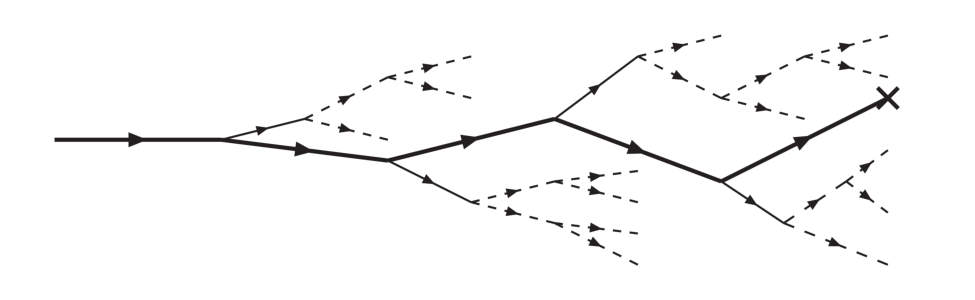
\includegraphics[scale= 0.8]{../Cap3/Fig_MC/isr}
\caption{ Evolution of the initial state. The bold line corresponds to the part that will undergo the hard process (represented by a cross). Thin lines represent the partons that can not recombine, while the dashed lines are fluctuations that may or may not recombine.  }
\label{isr}
\end{figure}

\begin{equation}
  \frac{d f_b(x, \:t)}{dt}= \sum_{ac} \int_x ^1 \frac{d x^{'}}{x^{'}} \: f_a(x^{'},t) \:\frac{\alpha_{abc}}{2\pi} \:P_{a \rightarrow bc} \:(\frac{x}{x^{'}}) \mbox{,}\end{equation}
where $f_{a,b}(x, \:t)$ are the parton PDFs  $a$, $b$, that which have $ x $ fraction of the incident and scale proton momenta $t=\mbox{ln}(Q^2/ \Lambda^2) $, instead $P_{a \rightarrow bc}$ is the kernel splitting function.\\
In the backward evolution the probability that the parton $ b $ has been generated from $ a $ in the interval between $ t $ and $ t-dt $ is given by:
\begin{equation}
d\mathcal{P}_{b}(t)=\frac{d f_b(x, \:t) }{ f_b(x, \:t)}= |dt| \sum_{ac}  \int  \frac{d x^{'}}{x^{'}} \frac{d f_a(x^{'}, \:t) }{ f_b(x, \:t)} \frac{\alpha_{abc}}{2\pi}          \:P_{a \rightarrow bc} \:(\frac{x}{x^{'}})      \mbox{,}\end{equation}
while the probability of non-division between the scale $t_{max}$ and $t<t_{max}$ is:
\begin{equation}
S_b (x,t,t_{max})=   \mbox{exp} \left( - \int_t ^{t_{max}} dt^{'} \sum_{ac}  \int  \frac{d x^{'}}{x^{'}} \frac{d f_a(x^{'}, \:t^{'}) }{ f_b(x, \:t^{'})} \frac{\alpha_{abc}}{2\pi}          \:P_{a \rightarrow bc} \:(\frac{x}{x^{'}}) \right)     \mbox{,}\end{equation} 
Finally the probability of combining $ b $ in $ a $ in the range between $ t $ and $ (t-dt) $ from is:
\begin{eqnarray}
d \mathcal{P}_{b}^{\mbox{\footnotesize{ISR}}}(t) &=& - \frac{d S_b (x,t,t_{max})}{dt} dt \nonumber \\
&=&  \sum_{ac}  \int  \frac{d x^{'}}{x^{'}} \frac{d f_a(x^{'}, \:t) }{ f_b(x, \:t)} \frac{\alpha_{abc}}{2\pi}          \:P_{a \rightarrow bc} \:(\frac{x}{x^{'}})  \cdot S_b (x,t,t_{max}) dt \end{eqnarray}
In this case the Sudakov  form factor is different respect to FSR as it contains the PDFs.
This means that the parton shower results do not depend only on the algorithm but also on the PDFs used.

\subsection*{Resummation} When calculating an observable predicted by QCD in a perturbative way, the expansion in powers of $ \alpha_S $ contains terms of the type $ \alpha_S^n L^k $ ($ k < 2n $), where $ L = \ln (q_{cut} / s) $, being $ q_{cut} $ the cut on resolvable emission. 
When we consider small values of  $q_{cut}$ the logarithm of the perturbative expansion becomes large and the  perturbative series diverges.
The main  perturbative order of the expansion is $n$  only if the successive terms of the series are negligible, however this is not guaranteed if there are high value of L. 
It is therefore necessary to consider the terms that have a high value of the logarithm. The study of these terms is called resummation and is done by putting the terms together in the perturbation series according to their degree of divergence:
$ \alpha_S ^ n L ^ {2n} $ are the leading log (LL) terms, $ \alpha_S ^ n L ^ {2n-1} $ are the next-to-leading log (NLL) terms, and so on. 
At the end  all $ \alpha_S $ orders terms are added. For many processes calculations are available at the NLL.
The parton shower approximate the effects of resuming at the NNLL. 

\subsection*{Merging among ME and PS}
The two different approaches for the  matrix element calculation  and for the parton shower have advantages and disadvantages. Regarding the ME we have:
\begin{itemize}
\item the LO matrix element calculations  can be performed exactly in the cases where there are many jet (of the order of six) in the final state,
\item a good description of separate partons is performed,
\item the perturbative calculations are correct,
\item however, the cross section diverges in the collinear and soft case, so an exhaustive description of the internal structure of jet is not possible.
\end{itemize}
On the other hand the PS:
\begin{itemize}
\item it is a universal approach that produces a realistic configuration of the partons,
\item the divergences, in the collinear limit, are treated with the introduction of the form factor of Sudakov. So we have an appropriate description of the jet evolution
\item however, the method fails when describing separate partons, since the collinear approximation in this case can not be valid.
\end{itemize}
Clearly the two methods are complementary and their merging is desirable. 
There are different approaches that combine ME with PS. The main difficulty is to cover the total phase space without overlaps or holes: we want to describe a process in which there are $ n $ well separated partons in the final state, using the LO matrix element  but  also including the  large logarithms resummation (LL, NLL) which is typical of the PS. A schematic description of the combination for four jet is given in Fig. \ref{merge}.
On the horizontal axis are the $ \alpha_S $ coupling orders, while on the vertical axis  the logarithm.
The PS includes the LL ($ m = 2n $) and the NLL ($ m = 2n-1 $) green circles (e.g. in the case of $ n = 2 $, $ m = $ 4, 3 the two circles  in green  marked as ``4'').
The circles that describe the event with four jet, when combining  the ME and  PS, are  green, the blue  and  three red  circles marked with the `` 4 ''.
The difficulty arises because the ME describes exactly all the circles marked with the `` 4 '': so if we simply sum up the two approaches 
we would  double counts these green circles.
\begin{figure}
\centering
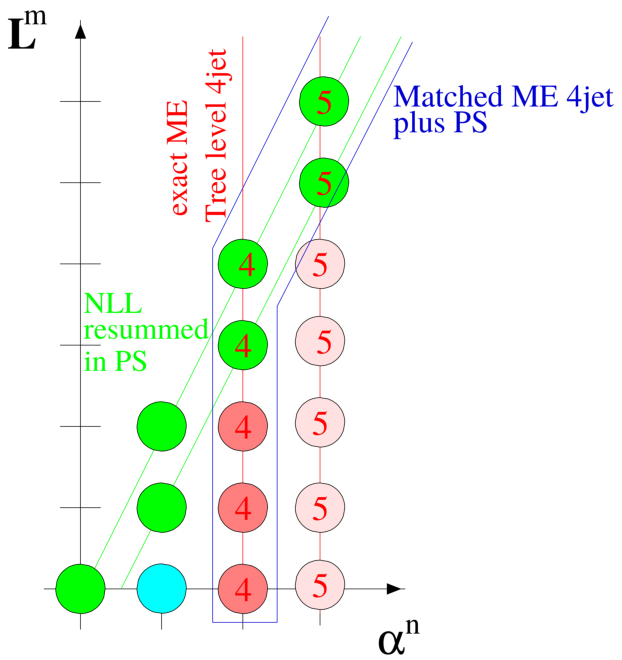
\includegraphics[scale= 0.7]{../Cap3/Fig_MC/merge}
\caption{ Merging among ME and PS.}
\label{merge}
\end{figure}
The most used approaches to merge the  ME and PS are:
\begin{itemize}
\item  parton shower reweight: the basic idea is to start from the process to the lowest order and then re-evaluate the output of the PS as if it had been produced by the ME. This approach does not change the cross section, which remains at the lowest order, but improves the population of the phase space \cite{ripesamento, ripesamento2}.
\item  CKKW prescription: the phase space is divided into two zones using $ k _ {\ perp} $ which is a measure of the cut $ Q_0 ^ 2 $: the region in which the jet is produced is filled with the ME, that of evolution with the PS \cite{ckkw, ckkw2}. 
\item The MLM prescription, which is also very widespread, is based on the same principle, but is implemented in a different way.
\end{itemize}


\section{Multiple Interaction}
Incident protons participating in the interaction are composed by  large number of partons (quark and gluons) that can interact independently with each other in addition to the hard process.
The total cross section for the QCD process $ 2 \rightarrow2 $ is dominated by the $t$-channel, so the cross section diverges as $ d p _ {\ perp} ^ 2 / p _ {\ perp} ^ 4 $ for $ p _ {\perp} \rightarrow 0 $ \cite{Sjostrand: 2006su}.
So when simulating a real event, in addition to the hard event, characterized by having large transverse transverse momentum, we must also take into account the additional collisions at small $ p _{\perp} $. If these occur independently then a Poisson distribution is expected, $ P_n = \langle n \rangle ^ n \mbox {exp} (- \langle n \rangle) / n! $. However, conservation of energy and momenta means that interactions are not effectively independent, thus suppressing the possibility, for $ p_{\ perp} \rightarrow 0 $, of having a high number of interactions.
It should also be noted that in order to eliminate the divergence it is necessary to introduce a cut-off value of the transverse pulse, below which no collisions are generated.



\section{Hadronization }
In this context, the process of hadronization is a particular model, used in event generators, which describes the transition from the final partonic state to the final hadron state, which is an  experimental observable. It is important to underline that this transition is treated in a phenomenological way and not by a rigorous approach. The two most important classes for tuning are the string model and the cluster model. The difference is that the former transforms the partonic systems directly into hadrons, while the second takes an intermediate step where it groups the objects to a scale of $ \sim 1 $ GeV.

\subsection*{String Model}
The Lund model is the most complete string model: we know from QCD that there is a linear confinement force between the partons that increases with distance. Consider, as an example, the final state in which there are two quark, $ q \bar{q} $. As the partons move away the color flow tube is stretched between $ q $ and $ \bar{q} $, Fig.~\ref{tubo} (a). The transverse dimensions of the tube are the typical dimension for the hadrons, therefore  about 1 fm.
If the tube is assumed to be uniform, the potential increases linearly, $ V (r) = \kappa r $, with $ \kappa \approx $ 1 GeV/fm, string constant.
\begin{figure}
\centering
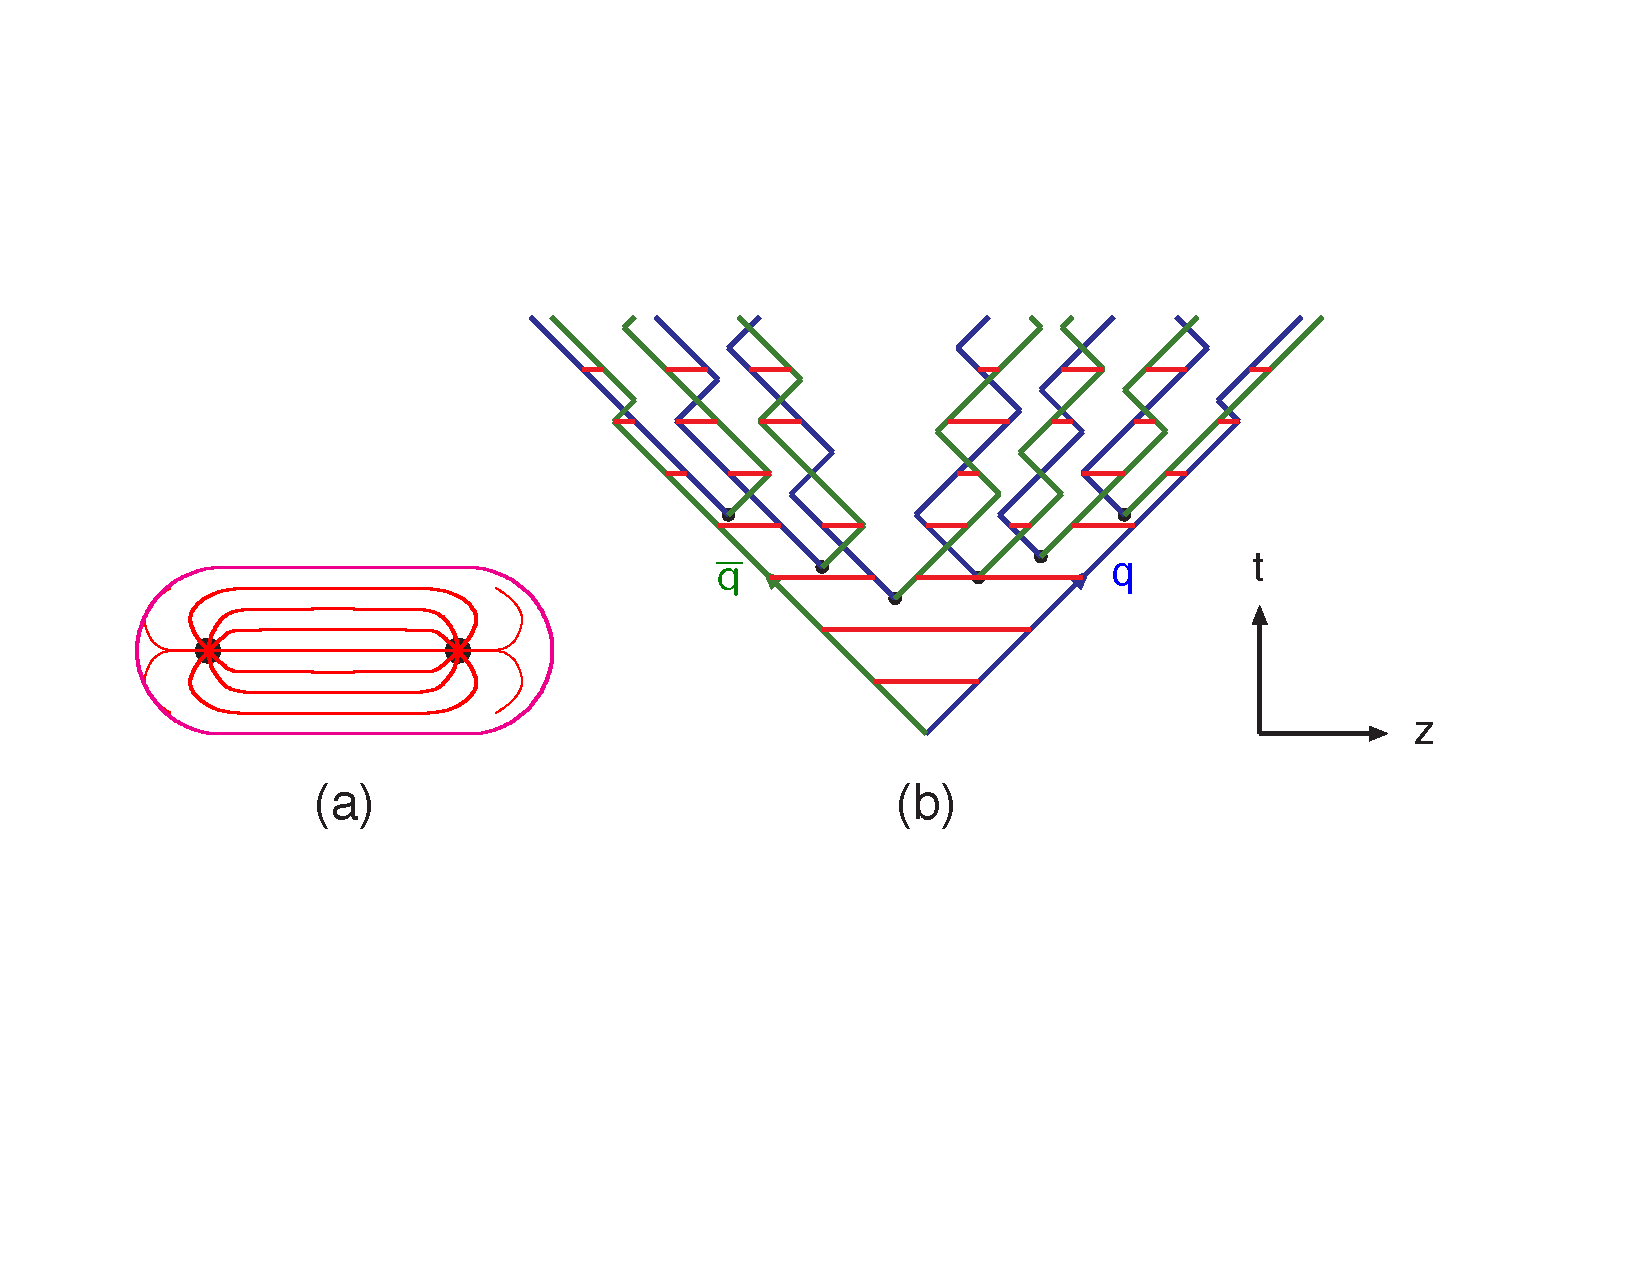
\includegraphics[scale= 0.5]{../Cap3/Fig_MC/stringone}
\caption{(a) The flow tube between a quark and an antiquark moving away. (b) Motion and breaking of a system string.}
\label{tubo}
\end{figure}
At short distances it would be necessary to introduce an additional Coulomb term, $ \sim \frac{\alpha_s}{r} $, however in the Lund model this term is  negligible.
As the quark and antiquark move away from the interaction vertex, the potential energy accumulated in the string increases until it breaks, giving rise to a pair $ q'  \bar{q}' $. So the system is divided into two new color singles $ q \bar{q} '$ and $ q' \bar{q} $. These two systems will move away  repeating the process below. The evolution of the system in space-time is represented in Fig.~\ref{tubo} (b).
At the end of the process  a serious of  $ q_i \bar{q_i} $ pairs are presented, each of which will form a hadron.
For now, only the case $ q \bar{q} $ has been considered. However, if more partons come from the interaction, the string model becomes more complicated. For an event in which there is an additional gluon, $ q \bar{q} g $, the string is stretched between $ q $ and $ g $ and between $ g $ and $ \bar{q} $, Fig. \ref{tubo3}.


\begin{figure}
\centering%
{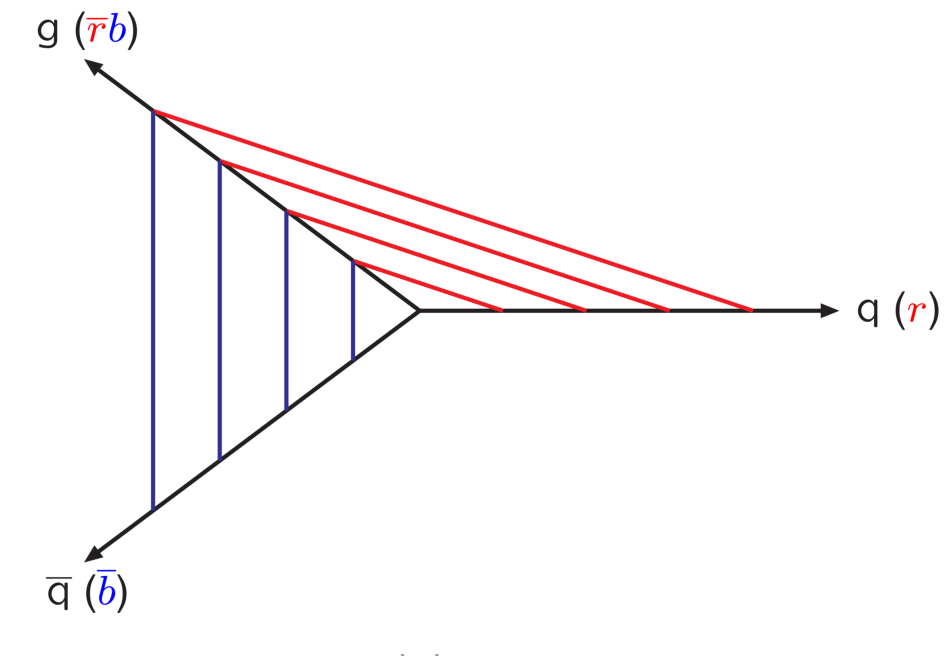
\includegraphics[scale= 0.5]{../Cap3/Fig_MC/stringtwo22}}
\caption{Motion of the string in the case $q \bar{q}g$.}
\label{tubo3}
\end{figure}

\begin{figure}
\centering%
\subfigure[]%
{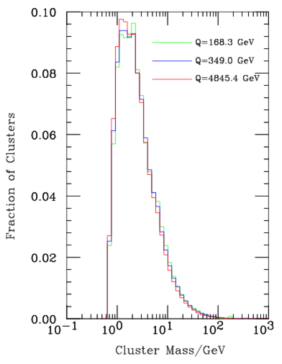
\includegraphics[scale= 1.5]{../Cap3/Fig_MC/split2}}
\subfigure[]%
{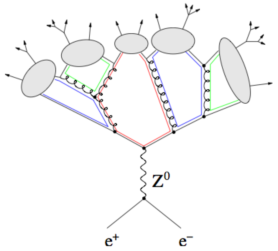
\includegraphics[scale= 1.4]{../Cap3/Fig_MC/split}}
\caption{(a)  Invariant mass distribution for singlets. (b) Parton shower structure in the cluster model.}
\label{tubo2}
\end{figure}


\subsection*{Cluster Model}  This  hadronization model  is based on the pre-confining property of the parton shower: 
the distribution of the invariant mass of a single pair of opposite-colored partons is the same at any $ Q^2 $ scale. 
The distribution increases rapidly at low value , Fig.~\ref{tubo2} (a). \\
In the model, the gluons from parton shower are represented by pairs of color-anticolor lines connected to the vertex. Each color line, near the cutoff, is connected to another colorless line present at the same scale. At this point the contiguous color/anticolor lines are interpreted, in the non-perturbative limit, as quark-antiquark pairs which give rise to mesons, which are observable objects in the final state.
This mechanism is represented in Fig.~\ref{tubo2} (b).

\section{Hadronic Decays and  Electromagnetic   Radiation.}
In the hadronization step, unstable hadrons which decay into other particles can be produced. So the final state  is the result of the convolution between the  hadronization  and the decay. The information necessary for the decay of unstable particles  is generally taken from the  ``Particle Data Book'' (PDG)~\cite{bib:pdg} which provides the properties (e.g. average life) of a large number of particles.
In general, in an event generator, it is necessary to choose which hadrons to include in the simulation and then select the possible decay channels. In addition to hadronic decays, it is also necessary to simulate the emission of electromagnetic radiation. The most common approach adopted is to use algorithms similar to those used to simulate the emission of QCD in parton shower.

\section{Jets} 
\label{rico_jet}
At the end of this process, after the hadronization and the decaying of  unstable particles it is still possible to estimate the four-momenta of the partons generated in the hard process as the direction and energy  of the jets  that are reconstructed  from the final state particles ~\cite{bib:run2jet}.
The jets are reconstructed by an algorithm that calculates the distance, $ d_ {ij} $, between two objects (particles or pseudo-jet ) defined as,
\begin{equation}
d_{ij}=\mbox{min}( k_{ti}^{2p}, k_{tj}^{2p})  \frac{\Delta_{ij}^2}{R^2} \mbox{,}\end{equation}
where $\Delta_{ij}^2=(y_i - y_j)^2+ (\phi_i - \phi_j)^2$ and $k_{ti}$, $y_i$ and $\phi_i$ are  the transverse momentum, the rapidity  e the azimutal angle of $i$ respectively. The constant $R$ is the radial parameter. The distance between  $ i $ and the beam  is also introduced , $d_{iB}=k_{ti}^{2p}$. \\
The algorithms proceed by calculating the minor distance $ d_{ij} $ between all the pairs of particles $ i $, $ j $. 
The four-momenta of the two particles with the smaller distance are added. The $ d_{iB} $ is evaluated for every $ i $ and if it is less than the distance $ d_{ij} $ with all other particles $ j $, $ i $,  than is is considered a jet and it is removed from list of objects present in the event.
Finally the distances are recalculated and this whole procedure is repeated until there are no more objects to be added.
For a value of $ p = -1 $ the algorithm is called anti-$k_t $ \cite{Cacciari:2008gp}. This is what has been used in this work, Sec.~\ref{jetr}.


\section{Main Monte Carlo generators }
For a proton-proton collision at the LHC, different Monte Carlo generators are available. Each of these has different methods for combining the ME with the PS.
A short introduction of  the main generators is given below. 
 
 
\subsection*{Madgraph\_aM{\footnotesize C@NLO}}
The \aMC \cite{bib:madgraph} approach is very ambitious, in fact the purpose of this generator is to calculate the cross section at the NLO including automatically both real and virtual contributions in the calculation. The  hard process is produced by the ME  while the soft emissions are added by the PS.
The first step is to compute the ME NLO corrections for a process involving $n$ partons. 
It results from  $n+1$ partons due to the real corrections and from $n$ partons due to the virtual corrections. 
As next step, it is evaluated  how the parton shower populates the phase space for $ n + 1 $ parton, excluding the Sudakov form factor. 
To get the state with $n+1$ partons, \aMC subtracts the PS  from the ME . 
The PS, without the Sudakov,  and the ME are in agreement in the soft and collinear limits, i.e. the singularities are deleted thus obtaining a finite value for the cross section for $ n $ and $ n + 1 $ partons. 
A technical problem arises in the collinear limit. Here, there is no certainty that the ME overhangs the PS everywhere. 
This problem is solved by introducing a fraction of negative-weight events, Fig.~\ref{weight}. 
Finally, the parton shower is applied, which includes the Sudakov factor and thus allows a finite and correct result to be obtained at the NLL. 
 \begin{figure}
\centering
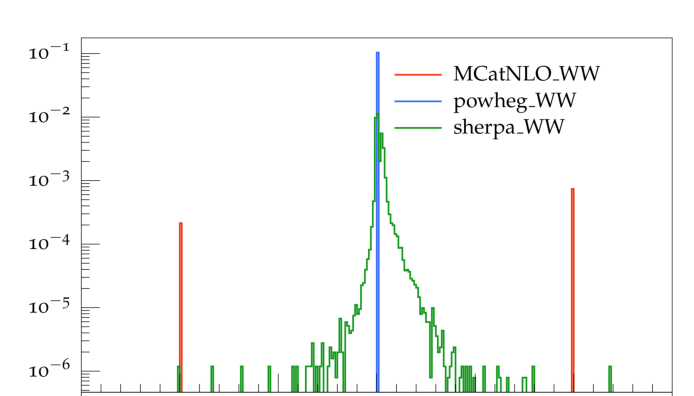
\includegraphics[scale= 0.7]{../Cap3/Fig_MC/weight}
\caption{Weight distribution, for different Monte Carlo generators, with cross section normalization of 1 fb$^{-1}$.}
\label{weight}
\end{figure}
 
\subsection*{P{\footnotesize OWHEG}} The idea behind P{\footnotesize OWHEG} \cite{Oleari:2010nx} is to generate the hardest radiation first, and then pass the event to the parton shower generator. In parton shower generators, the production, ordered in a transverse pulse, of the harshest radiation is always the first; so P{\footnotesize OWHEG} simply replaces this with the NLO emission.
In P{\footnotesize OWHEG} events are produced with a positive and constant weight (Fig.~\ref{weight}).
 
 
\subsection*{P{\footnotesize YTHIA}8 } P{\footnotesize YTHIA 8} \cite{bib:pythia} is a generator that can calculate the ME for processes with two particles or partons in the final state, but above all it generates the parton shower and the subsequent synchronization. The parton shower is ordered in a transverse impulse, $ p_T $, and the first issue is corrected with reweight method. For hadronization is used the Lund model.
 
 
\subsection*{S{\footnotesize HERPA}}  S{\footnotesize HERPA}  \cite{bib:sherpa} is a Monte Carlo generator that like PYTHIA8 provides a complete description of hadronic collisions, from the calculation of the matrix element, up to the stable particles. The parton shower includes both QCD and QED emissions, i.e. photons. It can calculate the ME for the main processes (eg $ gg \rightarrow H $) at the NLO and combine the ME with the PS. The code is written completely in C $ ++ $ language.




\section{Monte Carlo samples in High Mass Analysis}
\label{MSsample}
Several  Monte Carlo  generators were used in the searching of a high mass particle to simulated the signal and the backgrounds. 
All processes are simulated using the NNPDF3.0~\cite{Ball:2013hta,Ball:2011uy} parton distribution functions (PDF) for NLO ME generators,
while the LO version of the same PDF is used for LO ME generators. All the event generators are interfaced 
to \PYTHIA 8.1~\cite{Sjostrand:2007gs} for the showering of
partons and hadronization, as well as for including a simulation of the underlying event (UE) and multiple interactions (MPI)
based on the CUET8PM1 tune~\cite{Khachatryan:2015pea}. 
For all processes, the detector response is simulated using a detailed
description of the CMS detector, based on the \GEANT{}4 package~\cite{Agostinelli:2002hh}. 
The simulated samples are generated with distributions for the number of pileup interactions that are meant to roughly cover,
though not exactly match, the conditions expected for the different data-taking periods. In order to factorize these effects, 
the number of true pileup interactions from the simulation truth (as stored in the Monte Carlo)
is reweighted to match the data.
The re-weighting is propagated automatically to both the in-time pile up and the out-of-time one.
The pileup histogram for reweighting is calculated using the \emph{pileupCalc} tool as described in~\cite{puJSON}. 
Different calculations are used to obtain the cross sections for the all processes at 13\TeV. 
All simulated sample are summarized in Tab.~\ref{tab:wwl}.



%\hspace{-2cm}
\begin{table*}[htb]
\hspace{-1cm}
%\begin{center}
\footnotesize{
\begin{tabular}{@{}|l|c|c|c|@{}}
\hline
Process & Dataset Name & $\sigma\times$BR [pb] \\
\hline
Signal ggH &GluGluHToWWTo2L2NuM200-3000&Various \\
\hline
Signal VBF &VBFHToWWTo2L2NuM200-3000&Various \\

\hline
\ttbar$\rightarrow$\WW$b\bar{b}\rightarrow2l2\nu b\bar{b}$ & TTTo2L2Nu 13TeV-powheg  & 87.31 \\
\hline
\qqbar$\rightarrow$\WW$\rightarrow2l2\nu$ & WWTo2L2Nu 13TeV-powheg & 12.178 \\
\qqbar$\rightarrow$\WW$qq \rightarrow l\nu qq$  & WpWmJJ-QCD-noTop 13TeV-powheg & 0.59 \\
$gg\rightarrow$\WW$\rightarrow2l2\nu$ &  GluGluWWTo2L2Nu MCFM 13TeV & 0.5905 \\
\hline
Single top & ST tW top 5f inclusiveDecays &   35.85  \\
	&ST tW antitop 5f inclusiveDecays	&   35.85  \\
\hline
Drell-Yan	& DYJetsToTauTau\_13TeV-amcatnloFXFX-pythia8\_ext1 & 1867 \\
		& DYJetsToLL\_M-50\_TuneCUETP8M1\_13TeV-madgraphMLM-pythia8 &  6025.26	\\
		& DYJetsToLL\_M-50\_HT100to200\_madgraphMLM-pythia8 &  147.4  \\
		& DYJetsToLL\_M-50\_HT200to400\_madgraphMLM-pythia8 &  40.99  \\
		& DYJetsToLL\_M-50\_HT400to600\_madgraphMLM-pythia8 &  5.678  \\
		& DYJetsToLL\_M-50\_HT600toInf\_madgraphMLM-pythia8 &  2.198  \\
\hline
Multibosons	& WZTo2L2Q\_13TeV\_amcatnloFXFX\_madspin\_pythia8 &  5.5950 \\
		& ZZTo2L2Q\_13TeV\_amcatnloFXFX\_madspin\_pythia8 &  3.2210 \\
		& WWZ\_TuneCUETP8M1\_13TeV-amcatnlo-pythia8  &	0.1651 \\
		& WZZ\_TuneCUETP8M1\_13TeV-amcatnlo-pythia8 &  0.05565 \\
\hline




\end{tabular}
}
\caption{Simulated samples for \ttbar and \WW production.}
\label{tab:wwl}
%\end{center}
\end{table*}






\subsection*{Signal}  In order to perform the resonance search in a large part of the mass spectrum, several signal samples for the gluon-gluon fusion and the vector boson fusion mechanisms have been generated corresponding to different Higgs boson masses in the range between 200\GeV to 3\TeV. 
All signal samples have been simulated with \POWHEG v2~\cite{Nason:2004rx,Frixione:2007vw,Alioli:2010xd}, designed to describe the full NLO properties of these processes. In particular, for Higgs produced via gluon fusion~\cite{Alioli:2008tz}, and vector-boson-fusion (VBF)~\cite{Nason:2009ai},
the decay of the Higgs boson into two W boson and subsequently into leptons was done using JHUGen~\cite{jhugen}. 
The signals which correspond to a Higgs boson mass of 125\GeV have been simulated accordingly and are treated as backgrounds in the following analysis, including the associated production with a vector boson ($\mathrm{W^{+}H}$, $\mathrm{W^{-}H}$, ZH)~\cite{Luisoni:2013kna}, and gluon fusion produced ZH (ggZH). For associated production processes the Higgs boson decay was done via \PYTHIA 8.1~\cite{Sjostrand:2007gs}.
For Higgs signals, the cross sections used are the ones reported but the LHC Higgs Cross Section Working Group~\cite{temphiggsxsecs},
computed at NNLO and NNLL QCD and NLO EW for gluon fusion, and at NNLO QCD and NLO EW for the rest of the production modes.
The branching fractions are the ones reported in \cite{Heinemeyer:2013tqa}. 




\subsection*{The WW sample} The \WW production, irreducible background for the analysis, was simulated in different ways. 
\POWHEG v2~\cite{Melia:2011tj} was used for $q\bar{q}$  induced \WW in different decays. 
The cross section used for \WW processes produced via $q\bar{q}$ was computed at NNLO. 
The \WW, produced via gluon-gluon fusion, was generated, with and without Higgs diagrams, using \MCFM v7.0~\cite{Campbell:2013wga}. 
The cross section for normalizing \WW,  produced via \qqbar, was computed at next-to-next-to-leading order
(NNLO). The leading-order (LO) cross section for ggWW is obtained directly from \MCFM.
For gluon fusion, the difference between LO and NLO cross sections is significantly big.
A scale factor of 1.4 is theoretically calculated~\cite{Aaboud:2018jqu} and applied to the gg$\to$WW background. \\
In the analysis two different WW Monte Carlo samples are merged: the ``$WW \rightarrow 2l 2\nu$'' at NLO and the ``WW plus 2 quark'' at LO.  
The second sample,  ``WW plus 2 quark'' at LO, contains  final state with two quarks or a gluon-quark system: only the final state with two quarks interferes with the signal.
To avoid double count between the two sample a cut on di-jet mass at generator level, $mjj_{GenLev}$, is applied. 
In particular the sample ``$WW \rightarrow 2l 2\nu$'' at NLO is used for $mjj_{GenLev} <100$ GeV and the ``WW plus 2 quark'' at LO is adopted for $mjj_{GenLev} >100$ GeV.
The  distribution for the reco di-jet mass is shown in Fig.\ref{fig:WW}. In particular the red distribution correspond the ``$WW \rightarrow 2l 2\nu$ NLO'' sample with a cut of  $mjj_{GenLev} <100$, the blue distribution to  ``WW plus 2 quark'' with $mjj_{GenLev} >100$ GeV. The sum of the red and blue distributions is shown in black. There is a good agreement between  the black distribution and the ``$WW \rightarrow 2l 2\nu$ NLO'' without any  $mjj_{GenLev}$ distribution  in green.
\begin{figure}[htbp]
\centering
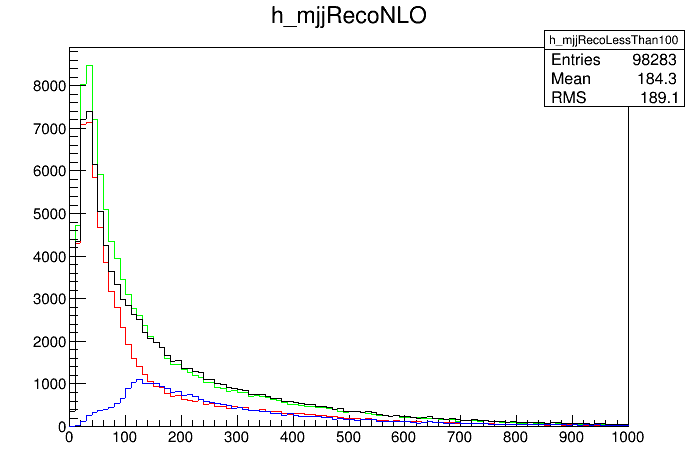
\includegraphics[width=0.6\textwidth]{../AN/Figs/WW_distribution}
\caption{ Distribution for $m_{jj}$ at RECO level for the merged WW sample.}
    \label{fig:WW}
\end{figure}




\subsection*{The Top sample}
In order to control the top quark background processes, the analysis is
performed in jet bins as described in Cap.~\ref{cap5}. The jet binning enhances the importance of logarithms of the jet \pt, spoiling the convergence of 
fixed-order calculations of the qq$\rightarrow$WW process and requiring the use of dedicated resummation techniques for an
accurate prediction of differential distributions~\cite{Meade:2014fca,Jaiswal:2014yba}.  
Since the \pt of the jets produced in association with the WW system is strongly correlated with its transverse momentum, 
\pt$^{WW}$,  the simulated qq$\rightarrow$WW events are reweighted  
to reproduce the \pt$^{WW}$ distribution from the \pt-resummed calculation.
A \ttbar  dilepton sample was also generated using \POWHEG v2. 
The cross sections of the different single top processes are estimated by the LHC Top Working group~\cite{singletop} at NLO.
The \ttbar cross section is also provided by the LHC Top Working group~\cite{topxsec}, and it is computed at NNLO, with NNLL soft gluon resummation. 


\subsection*{The DY sample}\label{sec:DY}
For the Drell-Yan backgrounds we use two different sets of samples. 
For the opposite flavore analysis (Sec~\ref{sec:OF}), selecting events with an
electron and a muon, a dedicated sample in which only the
$Z/\gamma^{*}\rightarrow{}\tau\tau\rightarrow{e\mu\nu\nu}$ decay is simulated.
For the same flavor analysis (Sec.~\ref{sec:SF}), in which pairs of electrons
or muons are selected, a soup of different $H_T$ binned DY samples is used. A
detailed study about this soup is given below.
Drell-Yan production of Z/$\gamma^{*}$ is generated using \MADGRAPH~\cite{Alwall:2014hca} and the cross section is scaled using a LO to NNLO k-factor equal to 1.23. 
Given the lack of MC statistics in the LO inclusive DY sample the
$H_\mathrm{T}$-binned samples are used. This helps increasing the MC
statistics especially in the VBF category of the same flavor analysis, which is characterized by large values of $H_\mathrm{T}$.
The LO inclusive sample is used for events with $H_\mathrm{T} < 100$\GeV and it has been merged to the other samples selecting events with $H_\mathrm{T}$ below 100\GeV using the parton level information. The cross sections of those samples have been scaled applying the LO to NNLO k-factor. In Fig.~\ref{fig:DY_HT} the $H_\mathrm{T}$ distribution of the sample after the merging is reported, showing a smooth transition between different $H_\mathrm{T}$ samples.
\begin{figure}[htbp]
\centering
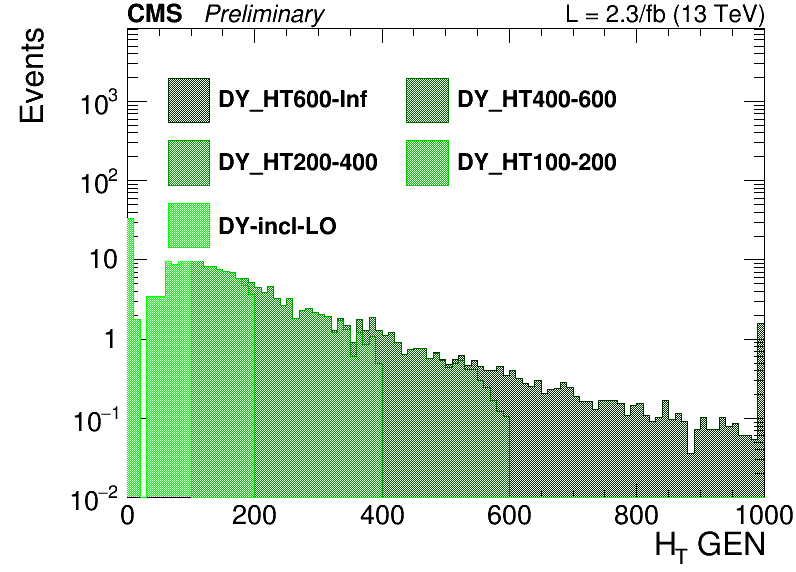
\includegraphics[width=0.6\textwidth]{../AN/Figs/log_c_incl_HTGen.png}
\caption{
    $H_\mathrm{T}$ distribution for the merged DY sample.}
    \label{fig:DY_HT}
\end{figure}
To further check the correct behaviour of the $H_\mathrm{T}$ binned samples we compared them to the inclusive LO sample, selecting only the events with a generator level $H_\mathrm{T}$ above 100\GeV. The comparison is done in a control region with two same flavor leptons with $\pt > 20$\GeV and $\mll > 50$\GeV, showing very good agreement between the two samples. The distributions of some variables are shown in Fig.~\ref{fig:inclDYvsHT}
\begin{figure}[htbp]
\centering
\subfigure[\mll]{
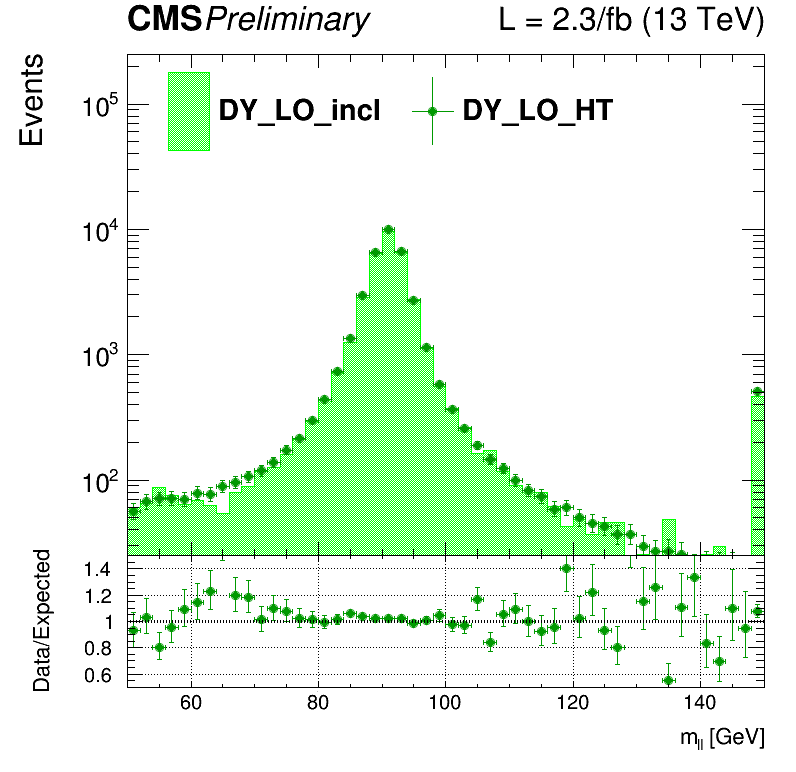
\includegraphics[width=0.45\textwidth]{../AN/Figs/DY/inclLOvsHT/log_cratio_dyee_13TeV_mll.png}
}
\subfigure[\ptll]{
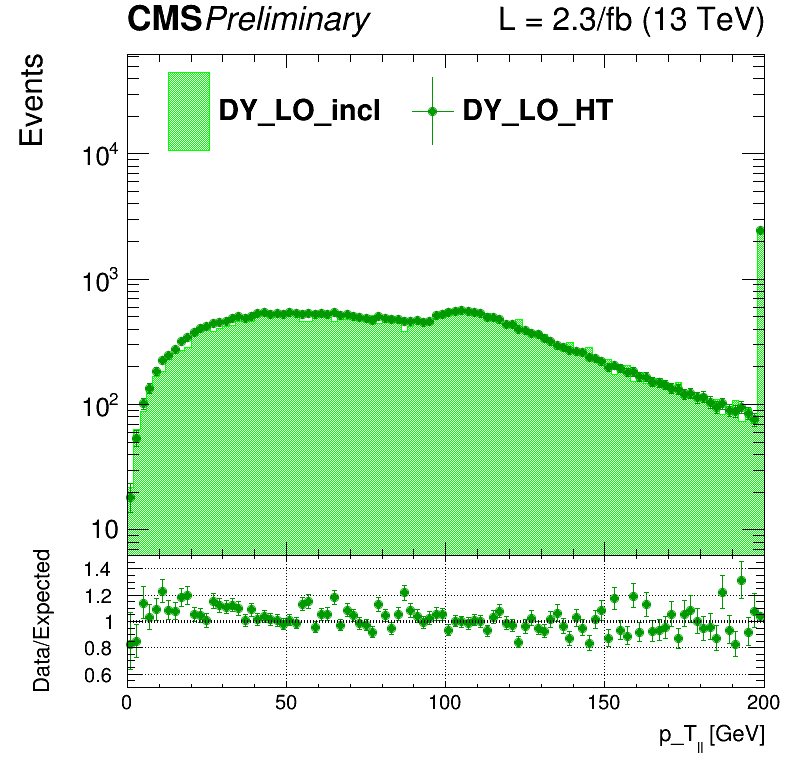
\includegraphics[width=0.45\textwidth]{../AN/Figs/DY/inclLOvsHT/log_cratio_dyee_13TeV_ptll.png}
}
\\
\subfigure[$\eta$ of leading lepton]{
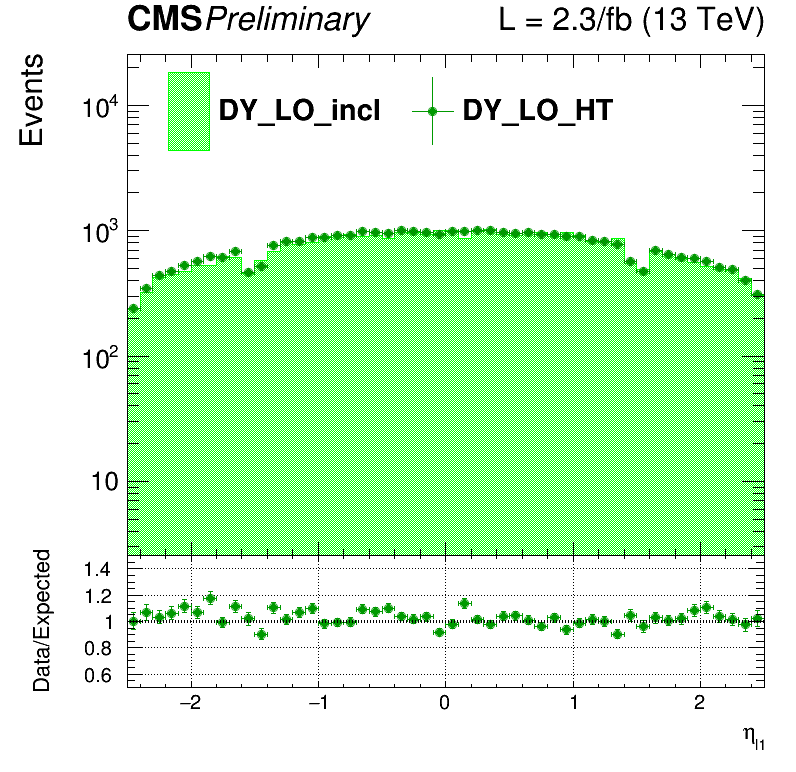
\includegraphics[width=0.45\textwidth]{../AN/Figs/DY/inclLOvsHT/log_cratio_dyee_13TeV_eta1.png}
}
\subfigure[$\eta$ of trailing lepton]{
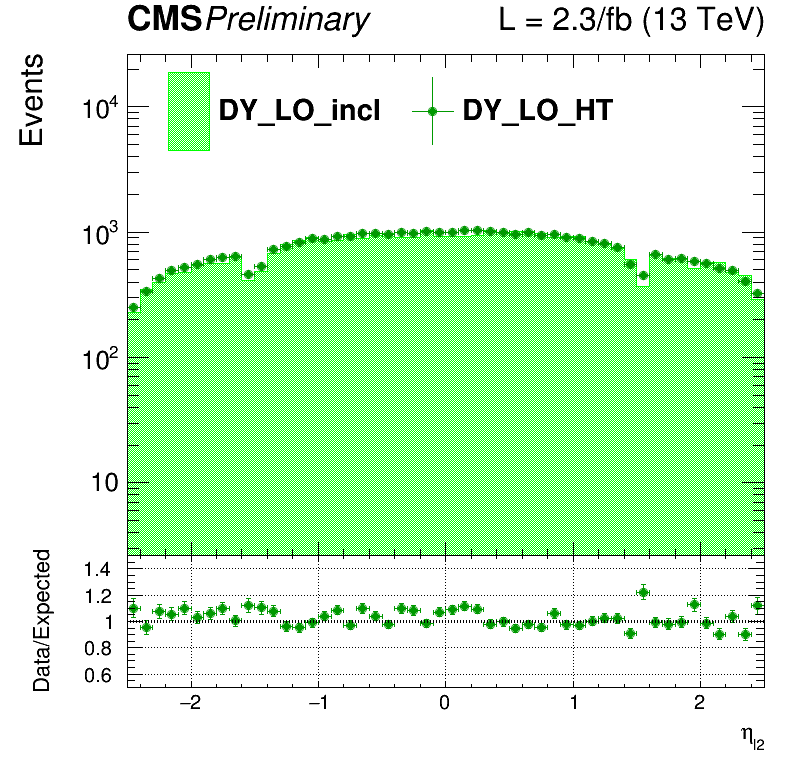
\includegraphics[width=0.45\textwidth]{../AN/Figs/DY/inclLOvsHT/log_cratio_dyee_13TeV_eta2.png}
}
\caption{
    Comparison between the inclusive LO DY sample and the $H_\mathrm{T}$ binned samples.}
    \label{fig:inclDYvsHT}
\end{figure}
To check the differences between the LO inclusive sample and the NLO sample simulated with \MCATNLO, the two samples have been compared in a same flavor control region and some variables of interest are shown in Fig.~\ref{fig:LOvsNLO}. The control region is defined requiring two same flavor leptons with $\pt > 20$\GeV and with $\mll > 50$\GeV.
\begin{figure}[htbp]
\centering
\subfigure[\mll]{
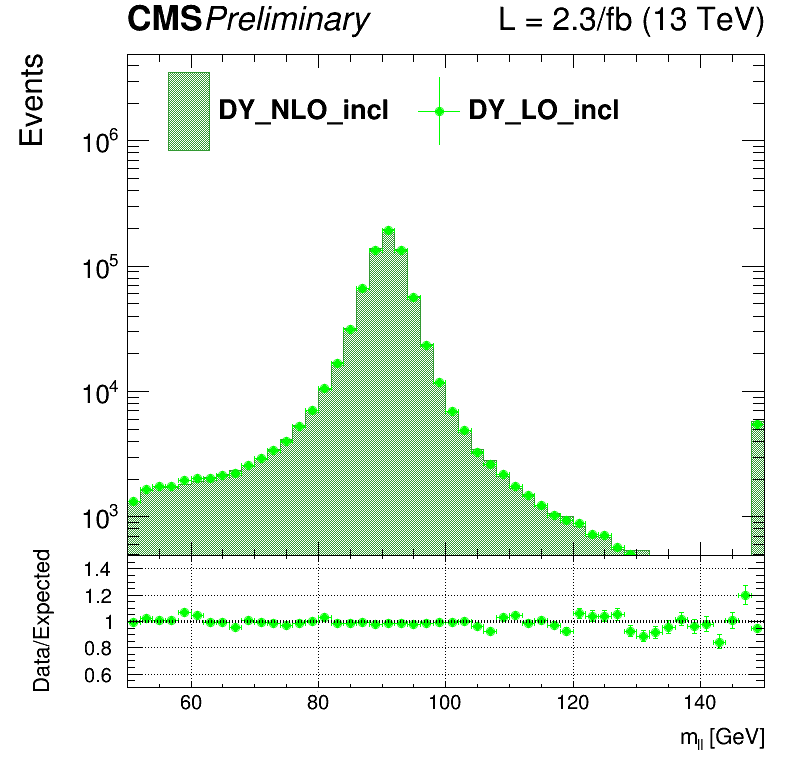
\includegraphics[width=0.45\textwidth]{../AN/Figs/DY/LOvsNLO/log_cratio_dyee_13TeV_mll.png}
}
\subfigure[\ptll]{
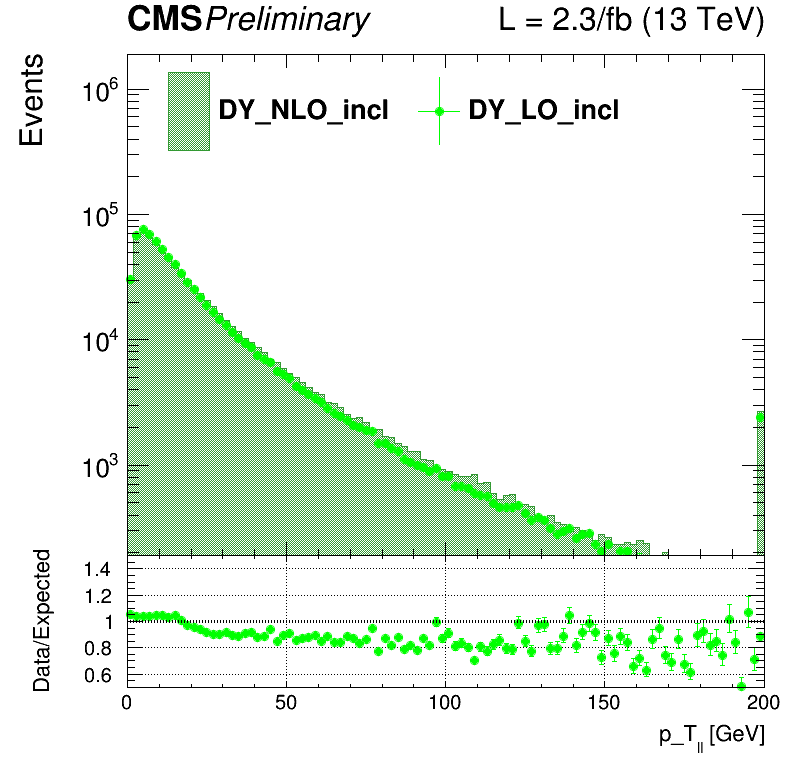
\includegraphics[width=0.45\textwidth]{../AN/Figs/DY/LOvsNLO/log_cratio_dyee_13TeV_ptll.png}
}
\\
\subfigure[$\eta$ of first lepton]{
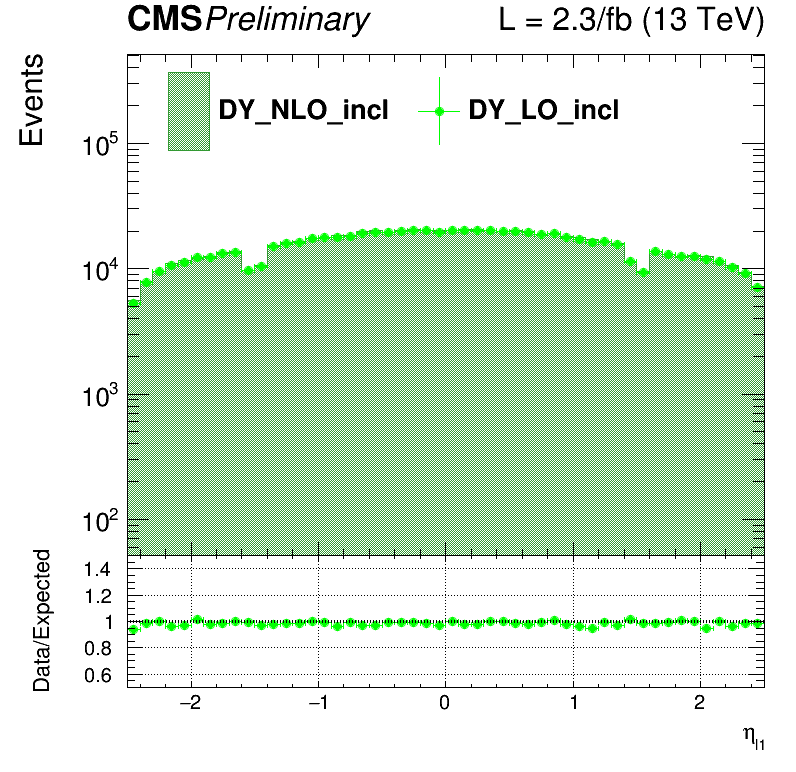
\includegraphics[width=0.45\textwidth]{../AN/Figs/DY/LOvsNLO/log_cratio_dyee_13TeV_eta1.png}
}
\subfigure[number of jets]{
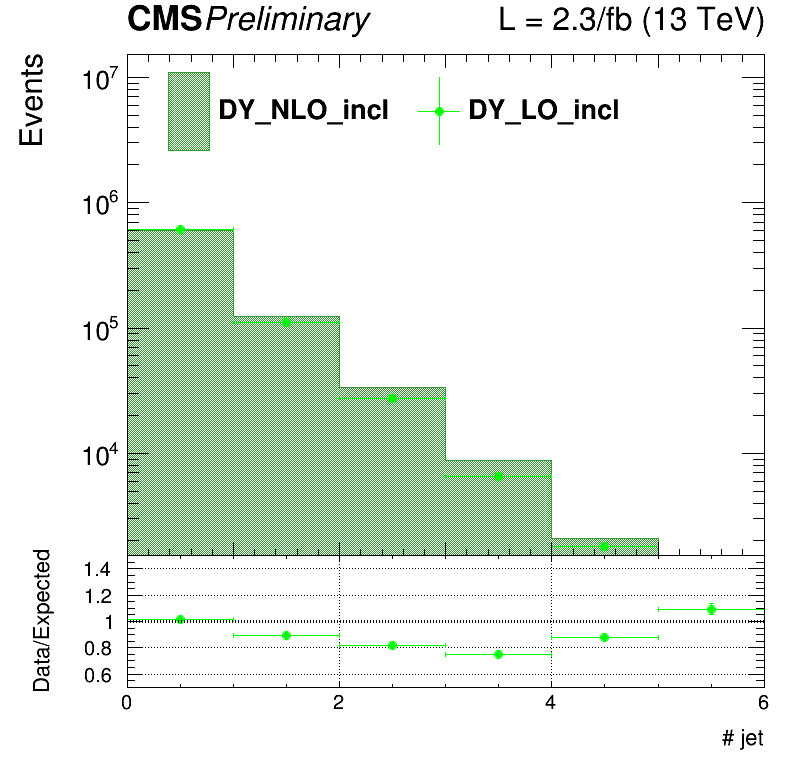
\includegraphics[width=0.45\textwidth]{../AN/Figs/DY/LOvsNLO/log_cratio_dyee_13TeV_njet.png}
}
\caption{
    Comparison between the LO and NLO DY samples.}
    \label{fig:LOvsNLO}
\end{figure}
The simulated samples are generated with distributions for the number of pileup interactions
that are meant to roughly cover, though not exactly match, the conditions expected for the
different data-taking periods. 
In order to factorize these effects, the number of true pileup interactions from the simulation truth is reweighted to match the data. 
The re-weighting is propagated automatically to both the in-
time pile up and the out-of-time one.
In Fig.~\ref{Fig:pu}, the effect of this reweighting on a sample enriched in Drell-Yan events is shown.
In order to select this sample, 
events with two electrons with \pt$> 25$~\GeV for the leading one and  \pt$>
13$~\GeV for the trailing one, are selected only if  $|\mll - m_Z| < 10$~\GeV. 

\subsection*{Other processes} Other multiboson processes, such as WZ,ZZ, and VVV (V=W/Z), are generated with a\MCATNLO and normalized
to the cross section obtained at NLO in generation.
The cross sections for the remaining processes were directly obtained from the generator itself.

